\documentclass[11pt,letterpaper,onecolumn,notitlepage]{article}
\usepackage[english]{babel}
\usepackage[compact]{titlesec}
\usepackage[titles]{tocloft}
\usepackage{%
  float,
  amssymb,
  amsmath,
  graphicx,
  fullpage,
  textcomp,
  gensymb,
  hyperref,
  listings,
  caption,
  sectsty,
  bm,
  times,
  parskip,
  empheq
}
\usepackage[framed,numbered,autolinebreaks,useliterate]{../sty/mcode}

\lstset{breakatwhitespace=false}

\newcommand{\figurepath}{../fig/hw4}
\newcommand{\codepath}{../include/code/hw4}

\sectionfont{\fontsize{16pt}{16pt}\selectfont\bfseries\sffamily}
\subsectionfont{\fontsize{13pt}{13pt}\selectfont\sffamily}
\subsubsectionfont{\fontsize{12pt}{12pt}\selectfont\sffamily}
\paragraphfont{\fontsize{11pt}{11pt}\selectfont\bfseries}

\makeatletter
\renewcommand\section{\@startsection{section}{1}{\z@}%
{-3.5ex\@plus-1ex\@minus-0.2ex}%
{1.0ex\@plus0.2ex}%
{\fontsize{12pt}{12pt}\selectfont\bfseries\sffamily}}
\makeatother

\makeatletter
\renewcommand\subsection{\@startsection{subsection}{1}{\z@}%
{-3.5ex\@plus-1ex\@minus-0.2ex}%
{0.5ex\@plus0.2ex}%
{\fontsize{10pt}{10pt}\selectfont\bfseries\sffamily}}
\makeatother

%------------------------------------------------------------------------
\setlength\cftparskip{-3pt}
\setlength\cftbeforesecskip{1pt}
\setlength\cftaftertoctitleskip{1pt}
\cftsetindents{figure}{0em}{1.5em}
\makeatletter
\renewcommand{\@dotsep}{4.5}
\renewcommand{\cftdotsep}{4.5}
\renewcommand{\cftsecdotsep}{4.5}
\renewcommand{\@tocrmarg}{4.55em}
\makeatother
\renewcommand\cftsecfont{\normalfont}
\renewcommand\cftsecpagefont{\normalfont}
\renewcommand{\cftsecleader}{\cftdotfill{\cftsecdotsep}}
%------------------------------------------------------------------------

\titleformat{\chapter}[display]{\huge\bf}{Lecture \thechapter}{0pt}{\Large}

\title{\textbf{Title}}
\author{Daniel Wiese \\ Department of Mechanical Engineering \\ Massachusetts Institute of Technology}
\date{\today}

\begin{document}

  \begin{titlepage}
    \begin{center}
      \rule{\linewidth}{0.01in} \\[0.25in]
      {\huge\bfseries 16.323 Optimal Control}\\[0.4cm]
      \rule{\linewidth}{0.01in} \\[0.25in]

      \textsc{\LARGE Problem Set 4}\\[0.15in]
      \large Due: Thursday, April 24, 2014 \\[1.0in]
      
\includegraphics[width=1.5in]{../fig/mit-seal.pdf}\\[3.0in]

      % Author and instructor
      \begin{minipage}{0.4\textwidth}
        \begin{flushleft} \large
          \emph{Author:}\\
          Daniel \textsc{Wiese}
          \vfill
        \end{flushleft}
      \end{minipage}
      \begin{minipage}{0.4\textwidth}
        \begin{flushright} \large
          \emph{Instructor:} \\
          Prof.~Steven \textsc{Hall} \\
        \end{flushright}
      \end{minipage} \\
      \vfill
    \end{center}
  \end{titlepage}

  \clearpage
  \section{Optimal Control with BVP4C}

  The problem is to find the optimal controller for the inverted pendulum, with dynamics given by

  \begin{equation*}
    \ddot{\theta}(t)=\sin(\theta(t))+u
  \end{equation*}

  $\theta=0$ corresponds to vertical.
  The cost functional to minimize is

  \begin{equation*}
    J=\int_{0}^{t_{f}}(\theta^{2}+\rho u^{2})dt
  \end{equation*}

  For the purposes of this problem, we will take $t_{f}=10$, $\rho=10$.

  \subsection*{Solution}

  This problem is described by the following equations

  \begin{align*}
    \dot{X} &= f(X,u) \\
    J       &= h+\int g dt
  \end{align*}

  where the state vector $X=[\;x_{1}\;x_{2}\;]^{\top}$ where $x_{1}=\theta$ and $x_{2}=\dot{\theta}$.
  In our problem the function $h$ for the terminal condition is

  \begin{equation*}
    \boxed{%
      h=0
    }
  \end{equation*}

  The dynamics are given by

  \begin{align*}
    \dot{x}_{1} &= f_{1} \\
    \dot{x}_{2} &= f_{2}
  \end{align*}

  where the function $f$ is written in component form as

  \begin{empheq}[box=\fbox]{alignat*=2}
    f_{1} &= x_{2} \\
    f_{2} &= \sin{}x_{1}+u
  \end{empheq}

  From the cost function we have

  \begin{equation*}
    \boxed{%
      g=x_{1}^{2}+\rho u^{2}
    }
  \end{equation*}

  Forming the Hamiltonian

  \begin{align*}
    H &= g+p^{\top}f \\
      &= g+p_{1}f_{1}+p_{2}f_{2} \\
      &= x_{1}^{2}+\rho u^{2}+p_{1}x_{2}+p_{2}(\sin x_{1}+u)
  \end{align*}

  Taking derivatives

  \begin{align*}
    H_{x}&=
    \begin{bmatrix}
      2x_{1}+p_{2}\cos x_{1} & p_{1}
    \end{bmatrix} \\
    H_{u}&=2\rho u+p_{2}
  \end{align*}

  And since $\dot{p}=-H_{x}^{\top}$ and $H_{u}=0$ we get the control is

  \begin{equation*}
    u=-\frac{p_{2}}{2\rho}
  \end{equation*}

  Putting everything together, the differential equations (state and costate) which describe the system are

  \begin{empheq}[box=\fbox]{alignat*=2}
    \dot{x}_{1} &= x_{2} \\
    \dot{x}_{2} &= \sin{}x_{1}-\frac{p_{2}}{2\rho} \\
    \dot{p}_{1} &= -2x_{1}-p_{2}\cos{}x_{1} \\
    \dot{p}_{2} &= -p_{1}
  \end{empheq}

  We have no terminal constraint, so the function $m$ is zero

  \begin{equation*}
    \boxed{%
      m=0
    }
  \end{equation*}

  and we augment the terminal cost with terminal constraint as

  \begin{equation*}
    w=h+\nu m
  \end{equation*}

  and so

  \begin{equation*}
    \boxed{%
      w=0
    }
  \end{equation*}

  And to find the boundary conditions we are given initial conditions on the state, and no final conditions.
  So we need to use final conditions on the costate equations which come from

  \begin{equation*}
    p(t_{f})=\biggr(\frac{\partial w}{\partial x}\biggr|_{t_{f}}\biggr)^{\top}
  \end{equation*}

  So this with the above that $w=0$ we get the final costate is zero.
  That is, the summary of all the boundary conditions is

  \begin{empheq}[box=\fbox]{alignat*=2}
    x_{1}(0)     &= \pi\\
    x_{2}(0)     &= 0 \\
    p_{1}(t_{f}) &= 0 \\
    p_{2}(t_{f}) &= 0
  \end{empheq}

  The scripts and functions which were used to solve this problem in \textsc{matlab} using \texttt{bvp4c.m} can be found in the appendix.
  A plot of the state and control histories is shown in Figure~\ref{fig:prob1} below.

  \begin{figure}[H]
    \centering
    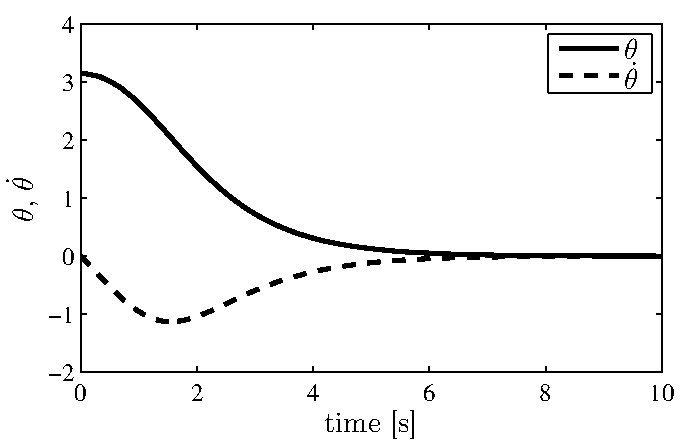
\includegraphics[width=3in]{\figurepath/prob1_state.pdf}
    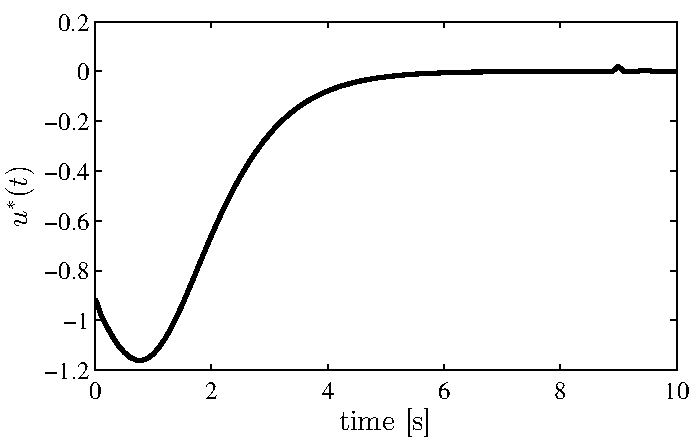
\includegraphics[width=3in]{\figurepath/prob1_control.pdf}
    \caption{State and control history plots for the pendulum system\label{fig:prob1}}
  \end{figure}

  \clearpage
  \section{Paper Summary: Survey of Numerical Methods for Trajectory Optimization}

  In the paper ``Survey of Numerical Methods for Trajectory Optimization'', the author, John T. Betts, reviews different approaches to solving the trajectory optimization problem, and summarizes the advantages and disadvantages of several methods.
  He starts with an overview of trajectory optimization and nonlinear programming (NLP) and discusses how the optimal control problem can be viewed as an extension of NLP.%
  He provides an overview of numerical schemes and discusses five widely used methods for solving the trajectory optimization problem.

  The general trajectory optimization problem is to determine the control input and parameters which will minimize a given performance index over a set of phases.
  The most general form is that where the objective function contains terms which depend on interval endpoints, as well as integrals over the time interval, and is known as the problem of Bolza.

  Nonlinear programming is introduced by considering the unconstrained minimization problem.
  This problem is extended to handle equality constraints using Lagrange multipliers, and finally to inequality constraints.
  The NLP problem is summarized simply as minimizing a given function $F(x)$ while imposing some inequality constraints on a function $c(x)$.
  The author gives a brief overview of approaches to solve this problem, including the use of penalty/barrier functions as mentioned in class.

  The optimal control problem is introduced as an extension of the nonlinear programming problem to an infinite number of variables.
  Using calculus of variations and augmented Lagrangians, this leads to a performance index which has continuous Lagrange multipliers, or costate variables.
  When optimality is sought by setting the first variation of this performance index to zero, the result is a set of necessary conditions which must be satisfied for optimality.
  This results in the Euler-Lagrange equations, including adjoint equations, control equations, and transversality conditions, which is a set of differential and algebraic equations, or DAE system.
  Solving such a system is a two-point boundary value problem.
  This problem is compared with the NLP problem, where the NLP Lagrange multipliers approximate the costate, and by using enough variables, the NLP solution approaches the optimal solution.

  Considering the equations developed using variational methods, the author describes several different methods to solve these equations numerically.
  These methods are: direct and indirect shooting method, multiple shooting method, and both direct and indirect transcription.
  The direct shooting method is widely used, and works well for launch vehicle and orbit transfer applications, due to the small number of NLP variables, but is difficult to apply when the number becomes large.
  The indirect shooting method is less applicable, as it is more prone to errors in the initial guess, and requires the derivation of the necessary conditions.
  The multiple shooting method seeks to improve the other shooting methods by splitting the trajectory into small segments and shooting over each segment.
  This results in increased robustness, and the ability to leverage parallel process for improved computation time, although this method is still somewhat sensitive to the initial guess.
  Indirect transcription, or collocation methods involve using a piecewise continuous polynomial to approximate the given function.
  As with other indirect methods, indirect transcription requires determining the costate equations, and can be difficult to use with path inequality constraints.
  Direct transcription does't require the costate equations or direct specification of path inequalities like in the indirect case.
  However, derivative information is required which is similar to the costate equations, and the direct method only approximates the solution of inequality constraints, often resulting in jump discontinuities in the control.

  In summary, given a trajectory optimization problem, the control designer should consider things such as the number of NLP variables required, how difficult it is to derive the costate equations, and whether path inequalities are present.
  Using this information will allow the control designer to pick the solution method which will likely work the best to solve the given problem.

  % One of the biggest setbacks to solving the trajectory optimization problem is the linear interpolation of table data.

  \clearpage
  \section{Optimal Control of Launch Vehicle}

  Consider the optimal control of thrust vector direction that maximizes the terminal velocity of a space launch vehicle in the rectilinear frame.
  The vehicle dynamics are represented as

  \begin{align*}
    \dot{u} &= a\cos\beta \\
    \dot{v} &= a\sin\beta \\
    \dot{x} &= u \\
    \dot{y} &= v
  \end{align*}

  where $(x,y)$ and $(u,v)$ denote the position and the velocity of the rocket with respect to a rectilinear inertial frame.
  The thrust acceleration $a$ is assumed to be a known function of time.
  The boundary conditions are given as:

  \begin{align*}
    u(t_{0})=v(t_{0})=x(t_{0})=y(t_{0}) &= 0 \\
    v(t_{f})                            &= 0 \\
    y(t_{f})                            &= z
  \end{align*}

  Also, the terminal time $t_{f}$ is given and $z$ is the altitude of the target orbit.

  \begin{enumerate}
    \item{Show that the optimal control law takes the form of}

    \begin{equation*}
      \tan\beta=\tan\beta_{0}-ct
    \end{equation*}

    where $\beta_{0}$ and $c$ are constant.
    This law is referred to as the \textit{linear tangent law}.

    \item{What happens if there exists the gravity described as}

    \begin{equation*}
    \dot{v}=a\sin\theta-G
    \end{equation*}

    with $g$ being constant?

    \item{%
      Use the numerical methods discussed in class to find the optimal control inputs and resulting path when $G=0$, $z=5000$ m, $a=2$ m/s$^2$, and $t_{f}=200$ sec.
      Compare the numerical and analytical solutions.
    }
  \end{enumerate}

  \subsection*{Solution 1.}

  As in the first problem, this problem is described by the following equations

  \begin{align*}
    \dot{X} &= f(X,u) \\
    J       &= h+\int g dt
  \end{align*}

  where the state vector $X=[\;x_{1}\;x_{2}\;x_{3}\;x_{4}\;]^{\top}$ where $x_{1}=u$, $x_{2}=v$, $x_{3}=x$, and $x_{4}=y$, and the input is $\beta=u$.
  In our problem the function $h$ for the terminal cost is to maximize the terminal velocity

  \begin{equation*}
    \boxed{%
      h=-x_{1}(t_{f})
    }
  \end{equation*}

  The dynamics are given by

  \begin{align*}
    \dot{x}_{1} &= f_{1} \\
    \dot{x}_{2} &= f_{2} \\
    \dot{x}_{3} &= f_{3} \\
    \dot{x}_{4} &= f_{4}
  \end{align*}

  where $a$ is a constant, the function $f$ is written in component form as

  \begin{empheq}[box=\fbox]{alignat*=2}
    f_{1} &= a\cos{}u \\
    f_{2} &= a\sin{}u \\
    f_{3} &= x_{1} \\
    f_{4} &= x_{2}
  \end{empheq}

  From the cost function we have

  \begin{equation*}
    \boxed{%
      g=0
    }
  \end{equation*}

  Forming the Hamiltonian

  \begin{align*}
    H &= g+p^{\top}f \\
      &= g+p_{1}f_{1}+p_{2}f_{2}+p_{3}f_{3}+p_{4}f_{4} \\
      &= p_{1}(a\cos u)+p_{2}(a\sin u)+p_{3}x_{1}+p_{4}x_{2}
  \end{align*}

  Taking derivatives

  \begin{align*}
    H_{x}&=
    \begin{bmatrix}
      p_{3} & p_{4} & 0 & 0
    \end{bmatrix} \\
    H_{u}&=-p_{1}a\sin u+p_{2}a\cos u
  \end{align*}

  Now we have the necessary conditions that $\dot{p}=-H_{x}^{\top}$ and $H_{u}=0$.
  This gives

  \begin{align*}
    \dot{p}_{1} &= -p_{3} \\
    \dot{p}_{2} &= -p_{4} \\
    \dot{p}_{3} &= 0 \\
    \dot{p}_{4} &= 0
  \end{align*}

  and

  \begin{equation*}
    p_{1}a\sin u=p_{2}a\cos u
  \end{equation*}

  Putting everything together, the differential equations (state and costate) which describe the system when $g=0$ are

  \begin{empheq}[box=\fbox]{alignat*=2}
    \dot{x}_{1} &= a\cos{}u \\
    \dot{x}_{2} &= a\sin{}u \\
    \dot{x}_{3} &= x_{1} \\
    \dot{x}_{4} &= x_{2} \\
    \dot{p}_{1} &= -p_{3} \\
    \dot{p}_{2} &= -p_{4} \\
    \dot{p}_{3} &= 0 \\
    \dot{p}_{4} &= 0
  \end{empheq}

  We have the terminal constraint

  \begin{equation*}
    \boxed{%
      m=x_{4}(t_{f})-z
    }
  \end{equation*}

  and we augment the terminal cost with terminal constraint as

  \begin{equation*}
    w=h+\nu m
  \end{equation*}

  and so

  \begin{equation*}
    \boxed{%
      w=-x_{1}(t_{f})+\nu(x_{4}(t_{f})-z)
    }
  \end{equation*}

  And to find the boundary conditions we are given initial conditions on the state, and final conditions on two of the states.
  So we need to use final conditions on the costate equations which come from the following, since $t_{f}$ is fixed

  \begin{equation*}
    p(t_{f})=\biggr(\frac{\partial w}{\partial x}\biggr|_{t_{f}}\biggr)^{\top}
  \end{equation*}

  So this with the above that $w=0$ we get the final costate is zero.
  That is, the summary of all the boundary conditions is

  \begin{empheq}[box=\fbox]{alignat*=2}
    x_{1}(0)     &= 0 \\
    x_{2}(0)     &= 0 \\
    x_{3}(0)     &= 0 \\
    x_{4}(0)     &= 0 \\[6pt]
    x_{2}(t_{f}) &= 0 \\
    x_{4}(t_{f}) &= z \\
    p_{1}(t_{f}) &= -1 \\
    p_{3}(t_{f}) &= 0
  \end{empheq}

  From the costate equations we know that $p_{3}$ and $p_{4}$ are constants.
  However, from the terminal boundary condition, we have that $p_{3}(t_{f})=0$ which means $p_{3}$ must be zero.

  \begin{align*}
    \dot{p}_{1} &= 0 \\
    \dot{p}_{2} &= -k
  \end{align*}

  So this gives that $p_{1}$ is constant and $p_{2}$ is a linear function of time.
  That is

  \begin{align*}
    p_{1} &= c_{1} \\
    p_{2} &= b_{2}t+c_{2}
  \end{align*}

  From above we have

  \begin{equation*}
    \tan\beta=\frac{p_{2}}{p_{1}}
  \end{equation*}

  and now we substitute in our known expressions for $p_{1}$ and $p_{2}$ to get the desired result.
  In particular, since $p_{1}$ is a constant, from the final condition we have $p_{1}=-1$ giving

  \begin{equation*}
    \tan\beta=-b_{2}t-c_{2}
  \end{equation*}

  And note to solve for $u=\beta$ from $\tan\beta=\frac{p_{2}}{p_{1}}$ since $p_{1}=-1$ when we take the inverse tangent, we need to consider 4-quadrant inverse tangent.

  \subsection*{Solution 2.}

  If the gravity term is included the equations are modified as

  \begin{equation*}
    \boxed{%
      h=-x_{1}(t_{f})
    }
  \end{equation*}

  \begin{empheq}[box=\fbox]{alignat*=2}
    f_{1} &= a\cos{}u \\
    f_{2} &= a\sin{}u-G \\
    f_{3} &= x_{1} \\
    f_{4} &= x_{2}
  \end{empheq}

  \begin{equation*}
    \boxed{%
      g=0
    }
  \end{equation*}

  Forming the Hamiltonian

  \begin{equation*}
    H=p_{1}(a\cos u)+p_{2}(a\sin u-G)+p_{3}x_{1}+p_{4}x_{2}
  \end{equation*}

  Taking derivatives

  \begin{align*}
    H_{x}&=
    \begin{bmatrix}
      p_{3} & p_{4} & 0 & 0
    \end{bmatrix} \\
    H_{u}&=-p_{1}a\sin u+p_{2}a\cos u
  \end{align*}

  Applying the necessary conditions we can see that the form of the solution is still the same.
  However, the presence of the gravity term $G$ will change the numerical values of the solution form.
  We had from before $p_{3}=0$, $p_{1}=-1$, and $p_{4}$ is constant, and $p_{2}$ depends on $p_{4}$.
  So the numerical value of $p_{4}$ due to gravity is different, and so the coefficients describing the linear function $p_{2}$ are different, resulting in different control history.
  The form will be the same though.

  \subsection*{Solution 3.}

  The equations and boundary conditions of part 1 were implemented in \textsc{Matlab} and simulated.
  The following plots show the trajectory of the spacecraft in $x$ and $y$, as well as the control history $\beta$ which is linear, as expected.

  \begin{figure}[H]
    \centering
    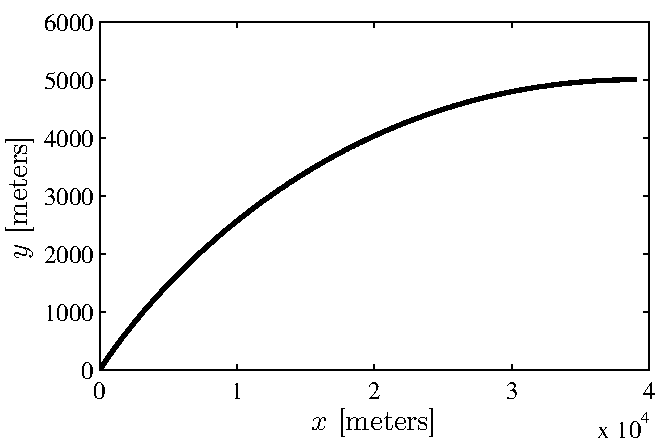
\includegraphics[width=3in]{\figurepath/prob3_traj.pdf}
    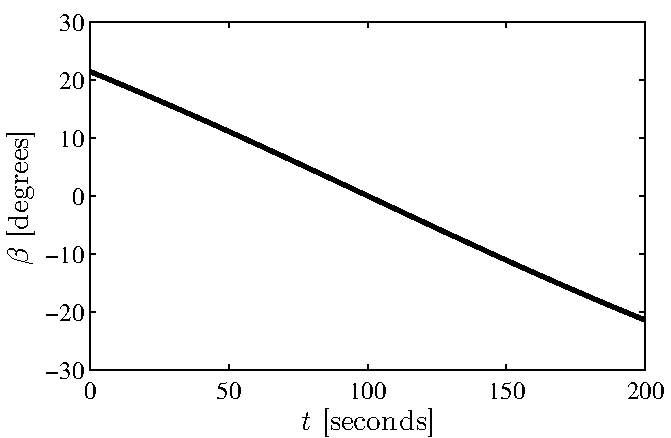
\includegraphics[width=3in]{\figurepath/prob3_control.pdf}
    \caption{State and control history plots for the pendulum system\label{fig:prob3}}
  \end{figure}

  \clearpage
  \section*{Code}

  \lstinputlisting{\codepath/p1_master.m}
  \lstinputlisting{\codepath/p1_initfun.m}
  \lstinputlisting{\codepath/p1_bcfun.m}
  \lstinputlisting{\codepath/p1_odefun.m}

  \lstinputlisting{\codepath/p3_master.m}
  \lstinputlisting{\codepath/p3_initfun.m}
  \lstinputlisting{\codepath/p3_bcfun.m}
  \lstinputlisting{\codepath/p3_odefun.m}

\end{document}
